\subsection{Progettazione di dettaglio e codifica}
\label{progettazione_di_dettaglio}
\textbf{Durata:} dal 2021\_03\_09 al 2021\_04\_30 \\
Il periodo inizia appena concluso il precedente e termina con la \glo{\textbf{RQ}}.
Le precondizioni sono:
\begin{itemize}
    \item Le postcondizioni del periodo precedente sono state soddisfatte.
\end{itemize}
Le postcondizioni sono:
\begin{itemize}
    \item Aggiornamento e correzione dei documenti già prodotti;
    \item Realizzazione dei diagrammi UML;
    \item Completamento codifica e relativa verifica;
    \item Redazione \textbf{manuale utente} e \textbf{manuale sviluppatore};
    \item Consegna dei documenti richiesti in entrata alla \textbf{RQ};
    \item Ultimata preparazione della presentazione da esporre in sede di revisione.
\end{itemize}
È composto da nuovi incrementi e nuove attività:
\begin{itemize}
    \item \textbf{Incremento e verifica dei documenti (dal 2021\_03\_09 al 2021\_03\_26):} i documenti già prodotti vengono migliorati e aggiornati se necessario ({\NdP}, {\PdP}, {\Glossario}, {\PdQ}, {\AdR});
    \item \textbf{Incremento e verifica delle attività (dal 2021\_03\_09 al 2021\_03\_17)}: viene migliorata l'attività di \glo{TB}, ampliando lo studio delle tecnologie mancanti e progettando ad alto livello come realizzare il prodotto finale;
    \item \textbf{Product Baseline (dal 2021\_04\_01 al 2021\_04\_13):} segue la \glo{TB} e a partire da quanto studiato e da quanto appreso con l'inizio dell'implementazione del prodotto viene individuato e confermato il materiale da presentare relativo a:
        \begin{itemize}
        	\item \textbf{Architettura della piattaforma};
            \item \textbf{Design pattern};
            \item \textbf{Diagrammi classi};
            \item \textbf{Diagrammi di sequenza}. 
        \end{itemize} 
    \item \textbf{Codifica (dal 2021\_03\_18 al 2021\_04\_29):} viene scritto il codice con relativa verifica. Questa attività, dato il modello di sviluppo scelto, verrà svolta prevedendo 3 incrementi diversi;
    \item \textbf{Manuale utente e manutentore(dal 2021\_04\_14 al 2021\_04\_29):} documenti redatti rispettivamente per indicare le istruzioni d'uso specifiche per l'utente e per supportare eventuali sviluppatori attraverso la descrizione dell'architettura del sistema.
\end{itemize}
\subsubsection{Incrementi del periodo}\label{IncrementiPDettaglio}
\begin{table}[H]
	\begin{center}
		\begin{tabular}{ |C{3cm} C{6cm} C{7cm}| }
			\rowcolor{darkblue} 
			\textcolor{white}{\textbf{Incremento}} & \textcolor{white}{\textbf{Obiettivi}} & \textcolor{white}{\textbf{Requisiti}} \\ \hline
			I dal 2021\_03\_09 al 2021\_03\_17& Miglioramento della documentazione già prodotta, ampliamento dello studio delle tecnologie, studio di \glo{design pattern}, diagrammi UML.  & - \\ \hline
			II dal 2021\_03\_18 al 2021\_04\_01 	& Correzione dei documenti post \glo{RP} e inizio sviluppo del codice. &  
			RFO1\_1 - RFO6\_1.1.5, RFO7\_2 \newline
			RFO8\_3, RFO10\_4, RFO11\_5 \newline
			RFO59, RFO60 \newline
			RFO61\_23 - RFO64\_23.3, RFO65\_24 \newline
			RF067, RFO68\_25 - RFO72\_25.4 \newline
			RFO73\_26, RFO74, RFO75, RFO11\_5, \newline 
			RFO12\_ 6 - RFO15\_ 6.3, RFO16 \newline RFO17, RFO18, RFO19\_7\newline RFO20\_8, RFO21\_9, RFO22\_10 \newline RFO23, RFO26, RFO27 \newline RFO29\_12, RFO66, RFO76 \newline RFO77, RFO78, RFO80 \\ \hline
			III dal 2021\_04\_01 al 2021\_04\_13	& Continuazione nello sviluppo del codice, preparazione alla \glo{PB}. & RFO81\_27 - RFO88\_27.7 \newline
			RFO89, RFO90\_28 - RFO97\_28.7 \newline
			RFO98\_29, RFO99\_30, RFO100\_31 \newline
			RFO101\_32, RFO102\_33 \newline
			RFO103\_34 - RFO107\_34.4, RFO108 \newline
			RFO109\_35 - RFO110\_35.1\newline
			RFO111\_36 - RFO112\_36.1, RFO113\_37 \newline RFO114\_38, RFO115, RFO25 \newline RFO30, RFO31\_13, RFO32\_13 \newline RFO33\_14, RFO34\_15, RFO35\newline  RFO36, RFO37\_16, RFO40\_16.1 \\ \hline
			IV dal 2021\_04\_14 al 2021\_04\_29 	& 
			Conclusione della redazione del codice con relative modifiche in seguito alla \glo{PB} e redazione dei manuali, preparazione alla \glo{RQ}. & RFO24, RFO38, RFO39\newline RFO40\_16.1,
			RFO41\_17 - RFO45\_17.1.4\newline
			RFO46\_18 - RFO50\_18.4, RFO51\_19 \newline
			RFO52, RFO53\_20, RFO54\_20 \newline
			RFO55\_21, RFO56\_22 - RFO58\_22.2 \newline
			RFO79, RFO116\_39, RFO117\_39 \newline RFO118\_40, RFO119, RFO120\_41 \newline
			RFO121\_42, RFO122\_43 - RFO126\_43.2.2 \\ \hline
		\end{tabular}
		\caption{Tracciamento incrementi-obiettivi}
	\end{center}
\end{table}

\newpage
\subsubsection{Ripianificazione attuata durante il periodo} \label{RipianificazionePDettaglio}
Data l'importanza di questo periodo il gruppo ha ritenuto necessario procedere ad una ripianificazione delle attività per poter affrontare la \glo{RQ} presentando un prodotto in uno stato avanzato del suo sviluppo, cosa non fattibile con le scadenze precedentemente individuate, per questo motivo si riporta il reale diagramma di Gantt utilizzato dal gruppo. Per i motivi precedentemente descritti il gruppo ha ritenuto di dover accedere a sportello alla \glo{RQ} in una data successiva rispetto a quanto stabilito inizialmente.
\subsubsection{Diagramma di Gantt: Progettazione di dettaglio e codifica} \label{GanttPDettaglio}
\begin{figure}[ht]
    \centering
    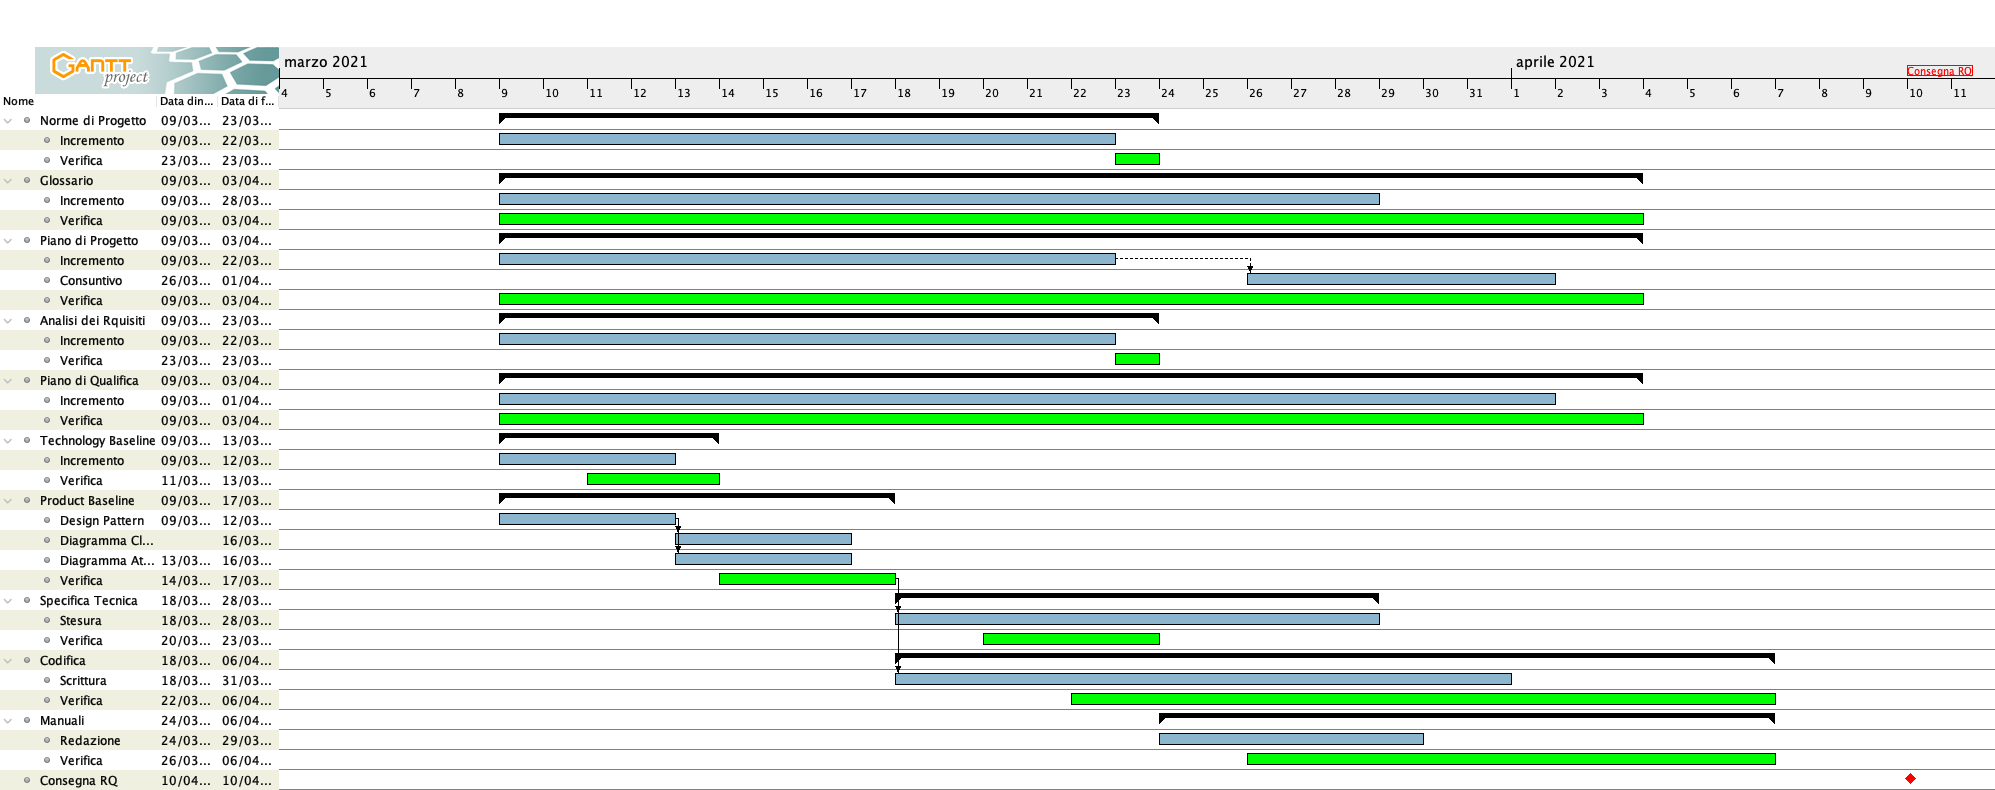
\includegraphics[width=\textwidth]{Immagini/GanttProgettazioneDiDettaglioECodifica}
    \caption{Diagramma di Gantt dell'attività di progettazione di dettaglio e codifica}
\end{figure}